% Include Preamble 
\documentclass[10pt,dvipsnames, aspectratio=169]{beamer}
\usetheme[progressbar=frametitle]{metropolis}
\usepackage[]{verbatim}\usepackage[]{}
\usepackage{booktabs}
\usepackage[scale=2]{ccicons}
\usepackage[misc]{ifsym}
\usepackage{wasysym}
\usepackage{listings}
\usepackage{xspace}
\usepackage{amsmath}
\usepackage{xcolor}
\usepackage{ragged2e}\justifying % for justify content % Customize 
\setlength{\parskip}{5pt} % vertical spacing between 2 paragraphs
\setbeamersize{text margin left=12mm, text margin right=12mm} 
\setbeamertemplate{frametitle}[default][left, leftskip=8mm]
%\usepackage[hidelink]{hyperref}
\newcommand{\themename}{\textbf{\textsc{metropolis}}\xspace}

% WARNING: Don't Touch,if you are not compfortable! 
\addtobeamertemplate{frametitle}{}{
%\begin{tikzpicture}[remember picture,overlay]
%\node[anchor=north east,yshift=2pt,xshift=-65pt] at (current page.north east) 
%{\includegraphics[height=.75cm]{img/elixir-portugal-white}};
%\node[anchor=north east,yshift=4pt] at (current page.north east) 
%{
\includegraphics[height=1cm]{img/hdro}};
%\end{tikzpicture}
}

% Title Page of Presentation 
% WARNING: Don't change logo, just write your details 
\title{Health Research ToolBox: A Step by Step Guide for Beginners}
\date{\today}
\author{ Jubayer Hossain 
	https://jhossain.me/}
\institute{Lead Organizer, Introduction to Scientific Computing for Biologists 
\\ Founder, \\ Center for Health Innovation, Research, Action and Learning}
\titlegraphic{\vspace{4cm}\hfill
\includegraphics[height=1cm]{img/jnulogo}}

\begin{document}
\maketitle
% Sectuion Title 
\section{Introduction to Hypothesis Testing}
% Slide - What is Inferential Statistics ?
\begin{frame}[t]{Inferential Statistics}
    \textbf{What is Inferential Statistics ?} \\
    \vspace{10px}
    Assess the strength of evidence for/against a hypothesis; evaluate the data.
    \begin{itemize}
 		\item Inferential statistical methods provide a confirmatory data analysis.
 		\item  Generalize conclusions from data from part of a group (sample) to the whole group (population)
 		\item Assess the strength of the evidence
 	    \item Make comparisons
 		\item Make predictions Inferential statistical methods divide into 2 categories.
    \end{itemize}

\end{frame}
%slide - 2 (Hypothesis Testing)
\begin{frame}[t]{Hypothesis Testing}
	 \textbf{Hypothesis Testing:} \\
	 Hypothesis testing is a formal procedure for investigating our ideas about the world using statistics. It is most often used by scientists to test specific predictions, called hypotheses, that arise from theories.
\end{frame}
%slide - 3 (Model Fitting)
\begin{frame}[t]{Model Fitting}
	\textbf{Model Fitting:} \\
	Model fitting is a measure of how well a statistical learning model generalizes to similar data to that on which it was trained. A model that is well-fitted produces more accurate outcomes.
\end{frame}
%slide - 4 (Inference)
\begin{frame}[t]{Inference}
	\textbf{What is Inference?} \\
	The process of drawing conclusions about population parameters based on a sample taken from the population. \\
	\begin{itemize}
		\item A sample is likely to be a good representation of the population.
		\item There is an element of uncertainty as to how well the sample represents the population.
		\item The way the sample is taken matters.
	\end{itemize}
\end{frame}
%slide -5 (Hypothesis)
\begin{frame}[t]{Inference}
	\textbf{What is Hypothesis?} \\
	\begin{itemize}
		\item Proposed explanation for a phenomenon.
		\item A hypothesis is an educated guess about something in the world around you. It should be testable, either by experiment or observation.
		\item Proposed explanation
		\item Objectively testable
		\item Singular - hypothesis
		\item Plural - hypotheses
	\end{itemize}
	\textbf{Examples}
		\begin{itemize}
		\item A new medicine you think might work.
		\item A way of teaching you think might be better.
		\item A possible location of new species.
	\end{itemize}
\end{frame}

%slide - 6 (hypothesis and study design)
\begin{frame}[t]{Hypothesis and Study Design}
	\textbf{Hypothesis:} seat belts decreases the fatality rate. \\
	\textbf{Study design:}  cross-sectional study of fatality outcome and seat-belt use of victims of motor vehicle accidents during a one-month time period in a large city
	\begin{figure}
		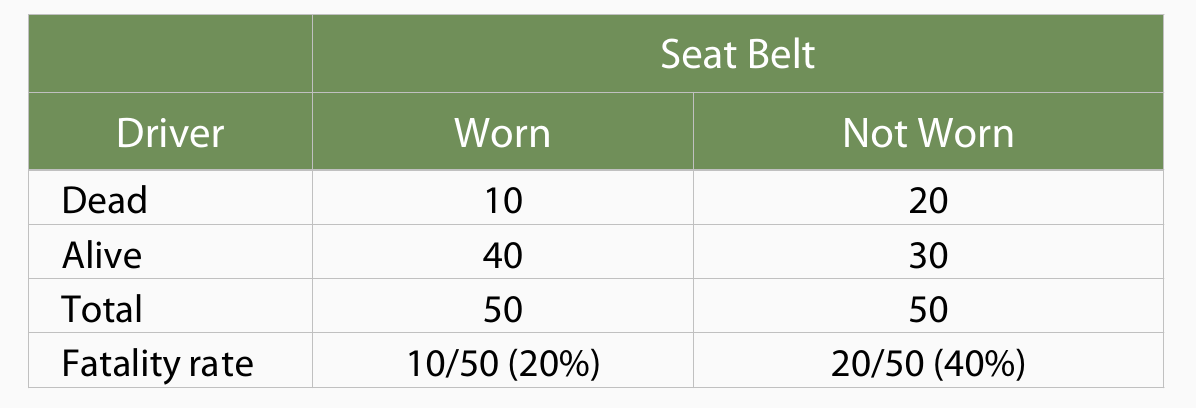
\includegraphics[width=300px]{img/seat_belt}
		%\caption{Jnu logo}
	\end{figure}
\end{frame}

%slide - 7 (hypothesis and study design)
\begin{frame}[t]{Hypothesis and Study Design (Con.)}
	\textbf{\large{Effect of Seat Belt Use on Accident Fatality}} \\
	\textbf{What is your conclusion?}  \\
	The fatality rate is: \\
	\begin{itemize}
		\item 40\% in the group of drivers who did not wear seat belts
		\item 20\% in drivers who did wear seat belts
	\end{itemize}
	Seat belts appear to save lives
\end{frame}

%slide - 8 (The Inferential Questions of Interest)
\begin{frame}[t]{The Inferential Questions of Interest}
	The inferential questions of interest are: \\
	\begin{itemize}
		\item Are results applicable to the population of all drivers? (generalization)
		\item Does wearing seat belts decreases fatality rate? (assess strength of evidence)
		\item Is the fatality rate of those not wearing seat belts higher than the fatality rate of those wearing seat belts? (comparison)
		\item How many lives can be saved by wearing seat belts? (prediction)
		\item Do other variables influence the conclusion?
		\item For example: the age of driver, alcohol use, type of car, speed at impact (ask more questions)
	\end{itemize}
	
\end{frame}
% Slide - 09 (Speed at Impact)
\begin{frame}[t]{Speed at Impact}
	\begin{figure}
		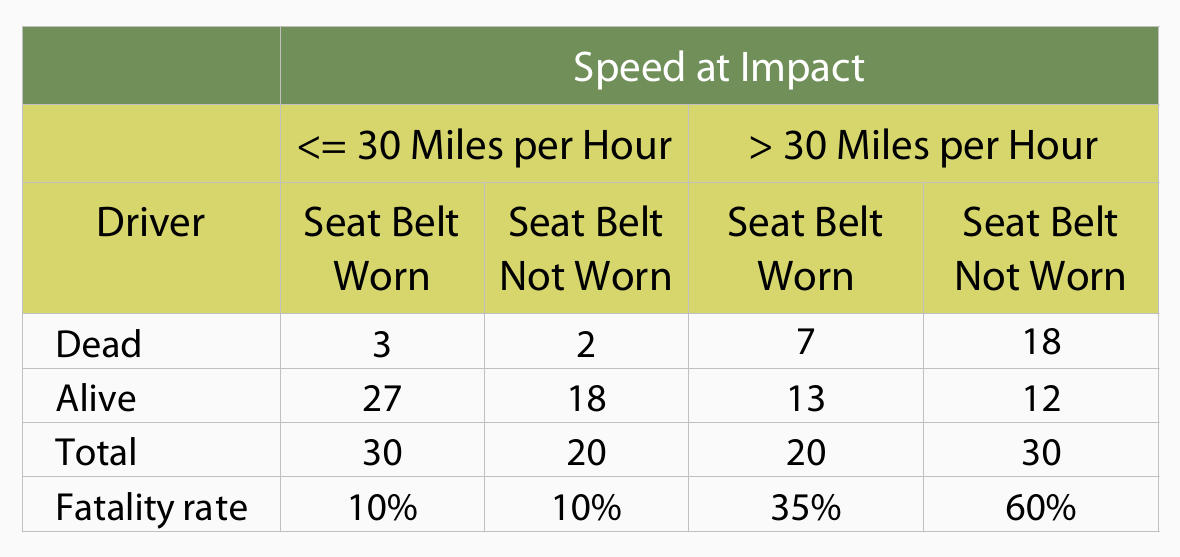
\includegraphics[width=12cm]{img/seat_belt2}
	\end{figure}
	
\end{frame}

% Slide - 10 (How Does This Influence Your Conclusion?)
\begin{frame}[t]{How Does This Influence Your Conclusion?}
	\begin{itemize}
		\item How does this influence your conclusion? \\
		- The fatality rate is 10\% at low-impact speeds regardless of seat-belt use.
		\item The fatality rate at high impact speeds is: \\
		-  60\% in drivers not wearing seat belts \\
		-  35\% in drivers wearing seat belts
	\end{itemize}
	
\end{frame}

% Slide - 11 (Null and Alternative Hypothesis)
\begin{frame}[t]{Null and Alternative Hypothesis}
	\begin{itemize}
		\item \textbf{Hypothesis 0 (H0):} \\
		Assumption of the test holds and is failed to be rejected at some level of significance.
		\item \textbf{Hypothesis 1 (Ha):} \\
		Assumption of the test does not hold and is rejected at some level of significance.
	\end{itemize}
	
\end{frame}

% Slide - 12 (Errors in the statistical tests)
\begin{frame}[t]{Errors in Statistical Tests}
	\begin{itemize}
		\item \textbf{Type I Error:} \\
		The incorrect rejection of a true null hypothesis or a false positive.
		\item \textbf{Type II Error:} \\
		The incorrect failure of rejection of a false null hypothesis or a false negativ.
	\end{itemize}
	\begin{figure}
		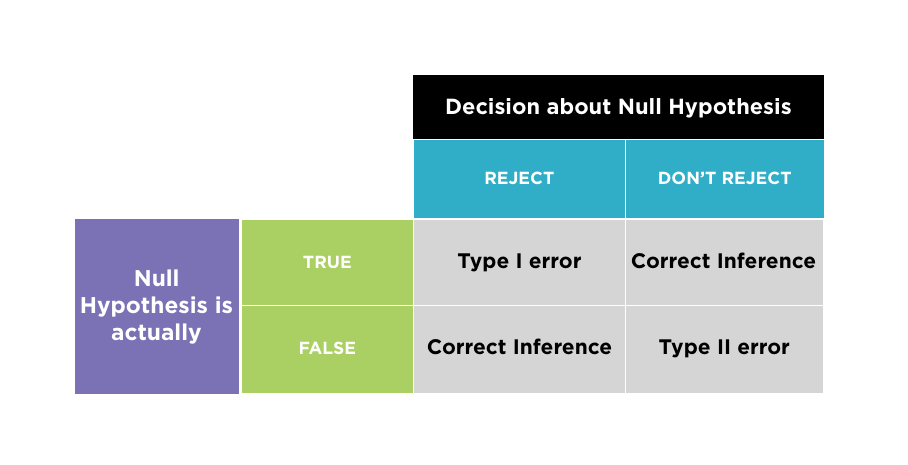
\includegraphics[width=11cm]{img/errors}
	\end{figure}
\end{frame}
% Slide - 13 (Alpha)
\begin{frame}[t]{Alpha ${\alpha}$}
	\begin{itemize}
		\item ${\alpha}$ is probability of rejecting H0 when H0 is true.
	 	\item ${\alpha}$ = Probability of Type-I error.
		\item Ranges from 0 to 1
		\item High ${\alpha}$ is not good
	\end{itemize}
\end{frame}
% Slide - 14 (p-value)
\begin{frame}[t]{P-value}
		In statistics, the p-value is the probability of obtaining results at least as extreme as the observed results of a statistical hypothesis test, assuming that the null hypothesis is correct. \\
		Generally cut off value of alpha 0.05. \\
	\begin{itemize}		
		\item If p-value \textgreater alpha: Fail to reject the null hypothesis (i.e. not significant result).
		\item If p-value \textless= alpha: Reject the null hypothesis (i.e. significant result).
	\end{itemize}
\end{frame}

% Slide - 15 (hypothesis testing process)
\begin{frame}[t]{Hypothesis Testing Process  (Con..)}
	\begin{itemize}	
		%Step	
		\item \textbf{Step-1: } Null Hypothesis H0 \\
		${\rightarrow}$ True until proven false \\
		${\rightarrow}$ Usually posits no relationship
		%Step
		\item \textbf{Step-2: } Select Test \\
		${\rightarrow}$ Pick from vast library \\
		${\rightarrow}$ Know which one to choose
		%Step
		\item \textbf{Step-3: } Significance Level \\
		${\rightarrow}$	Usually 1\% or 5\%  \\
		${\rightarrow}$ What threshold for luck?
	
	\end{itemize}
\end{frame}
% Slide - 16 (hypothesis testing process)
\begin{frame}[t]{Hypothesis Testing Process (Con..)}
	\begin{itemize}	
		%Step
		\item \textbf{Step-4: } Alternative Hypothesis \\
		${\rightarrow}$ Negation of null hypothesis \\
		${\rightarrow}$ Usually asserts specific relationship
		%Step
		\item \textbf{Step-5: } Test Statistic \\
		${\rightarrow}$ Convert to p-value \\
		${\rightarrow}$ How likely it was just luck?
		%Step
		\item \textbf{Step-6: } Accept or Reject \\
		${\rightarrow}$	Small p-value? Reject H0  \\
		${\rightarrow}$ Small: Bellow significance level
		
	\end{itemize}
\end{frame}

% Slide - 17 (hypothesis testing process)
\begin{frame}[t]{Hypothesis Testing Process}
	\begin{figure}	
	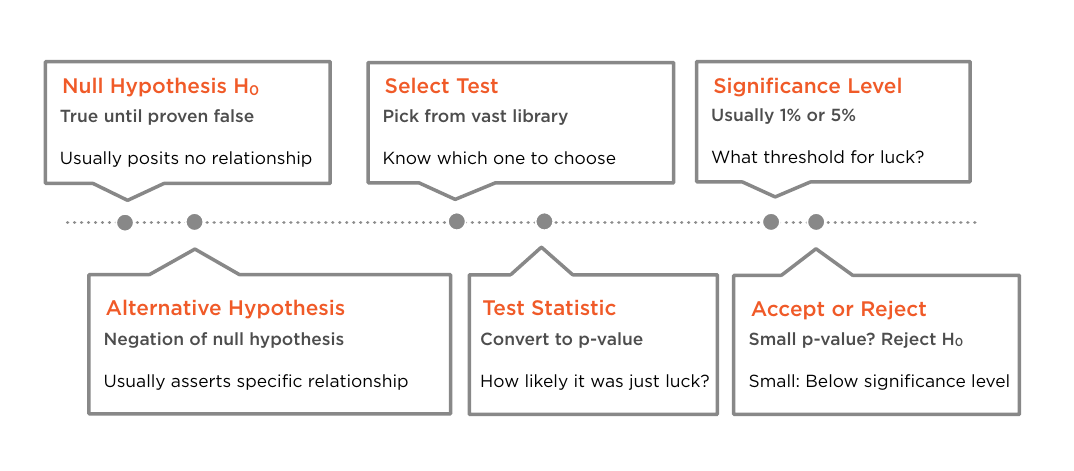
\includegraphics[width=12cm]{img/hypothesis}
	\end{figure}
\end{frame}


% Sectuion Title 
\section{Common Statistical Tests}
% Slide - 18 (Variable Distribution Type Tests)
\begin{frame}[t]{Variable Distribution Type Tests (Gaussian)}
	\begin{itemize}	
		\item Shapiro-Wilk Test
		\item D’Agostino’s $k^{2}$ Test
		\item Anderson-Darling Test
	\end{itemize}
\end{frame}

% Slide - 19 (Variable Relationship Tests)
\begin{frame}[t]{Variable Relationship Tests (correlation)}
	\begin{itemize}	
		\item Pearson’s Correlation Coefficient
		\item Spearman’s Rank Correlation
		\item Kendall’s Rank Correlation
		\item Chi-Squared Test
	\end{itemize}
\end{frame}

% Slide - 20 (Compare Sample Means)
\begin{frame}[t]{Compare Sample Means (parametric)}
	\begin{itemize}	
		\item Student’s t-test
		\item Paired Student’s t-test
		\item Analysis of Variance Test (ANOVA)
		\item Repeated Measures ANOVA Test
	\end{itemize}
\end{frame}


% Slide - 21 (Compare Sample Means)
\begin{frame}[t]{Compare Sample Means (nonparametric)}
	\begin{itemize}	
		\item Mann-Whitney U Test
		\item Wilcoxon Signed-Rank Test
		\item Kruskal-Wallis H Test
		\item Friedman Test
	\end{itemize}
\end{frame}
% Slide - 22 (Statistical Test Selection)
\begin{frame}[t]{Statistical Test Selection}
	\begin{itemize}	
		\item Mann-Whitney U Test
		\item Wilcoxon Signed-Rank Test
		\item Kruskal-Wallis H Test
		\item Friedman Test
	\end{itemize}
\end{frame}

%slide - 23 (statistical test selection)
\begin{frame}[t]{Statistical Test Selection}
	\begin{tabular}{l l}
		
		\textbf{What we observe in our sample data} & \textbf{Is it real?(statistical test)} \\
		\hline
		1 categorical variable & 1 sample proportion test  \\
		2 categorical variables & chi squared test \\
		1 numeric variable	& t-test \\
		1 numeric and 1 categorical variable & t-test or ANOVA \\
		more than 2 categorical variables & ANOVA \\
		2 numeric variables & correlation test \\
		
	\end{tabular}

\end{frame}

%slide - 22 (reference)
\begin{frame}[t]{Reference}
	\textbf{For learning more, visit -} \\
	1. https://machinelearningmastery.com/statistical-hypothesis-tests/   \\
	
	2. https://www.statisticshowto.com/probability-and-statistics/hypothesis-testing/
\end{frame}

% Thank you slide 
\plain{Thank You\\ \ \\ \Huge{\smiley}}

\end{document}